\documentclass{article}
\usepackage[italian]{babel}
\usepackage{geometry}
\usepackage{amsmath}
\usepackage{amssymb}
\usepackage{graphicx}
\usepackage{xcolor}
\usepackage[dvipsnames]{xcolor}
\usepackage{ulem}
\usepackage{listings}
\usepackage{array}
\usepackage{float}

\let\olditemize\itemize
\renewcommand\itemize{\olditemize\setlength\itemsep{0em}}

\definecolor{codegreen}{rgb}{0,0.6,0}
\definecolor{codegray}{rgb}{0.5,0.5,0.5}
\definecolor{codepurple}{rgb}{0.58,0,0.82}
\definecolor{backcolour}{rgb}{0.95,0.95,0.92}

\lstdefinestyle{mystyle}{
    backgroundcolor=\color{backcolour},   
    commentstyle=\color{codegreen},
    keywordstyle=\color{magenta},
    numberstyle=\tiny\color{codegray},
    stringstyle=\color{codepurple},
    basicstyle=\ttfamily\footnotesize,
    breakatwhitespace=false,         
    breaklines=true,                 
    captionpos=b,                    
    keepspaces=true,                 
    numbers=left,                    
    numbersep=5pt,                  
    showspaces=false,                
    showstringspaces=false,
    showtabs=false,                  
    tabsize=2
}

\lstset{style=mystyle}

\title{Assignment 2}
\author{\footnotesize Barletta Alessio (5686474)
Sacco Daniele (5616921)
Scaffai Daniele (5658260)
Vaccarecci Lorenzo Livio (5462843)\normalsize}
\date{}

\begin{document}

\maketitle

\section{Sonarlint}
\subsection{Cart.java}
Porzione di codice:
\begin{lstlisting}[language=Java]
if (quantity > 0)
    products.put(product, products.getOrDefault(product, 0) + quantity);
    else 
products.put(product, products.getOrDefault(product, 0));
\end{lstlisting}
Tipologia: Maintainability\\
Correzione:
\begin{lstlisting}[language=Java]
public void addProduct(Product product, int quantity) {
    if (quantity > 0)
        products.put(product, products.getOrDefault(product, 0) + quantity);
    else 
        products.put(product, products.getOrDefault(product, 0));
}
\end{lstlisting}
\vspace{.5em}\hrule\vspace{.5em}
Porzione di codice \texttt{updateProductQuantity}:
\begin{lstlisting}[language=Java]
if (products.containsKey(product)==true)
    if (quantity <= 0) 
        removeProduct(product);
    else 
        products.put(product, quantity);
\end{lstlisting}
Tipologia: Maintainability\\
Correzione:
\begin{lstlisting}[language=Java]
public void updateProductQuantity(Product product, int quantity) {
    if (products.containsKey(product)) {
        if (quantity <= 0) 
            removeProduct(product);
    }
    else { 
        products.put(product, quantity);
    }
}
\end{lstlisting}
\vspace{.5em}\hrule\vspace{.5em}
Porzione di codice \texttt{getProducts}:
\begin{lstlisting}[language=Java]
return new HashMap<Product, Integer>(products);
\end{lstlisting}
Tipologia: Maintainability\\
Correzione: 
\begin{lstlisting}[language=Java]
public Map<Product, Integer> getProducts() {
    return new HashMap<>(products);
}
\end{lstlisting}
\vspace{.5em}\hrule\vspace{.5em}
Porzione di codice:
\begin{lstlisting}[language=Java]
if(this.calculateTotal() >= cart1.calculateTotal() && this.calculateTotal() >= cart2.calculateTotal())
    return true;
else 
    return false;
\end{lstlisting}
Tipologia: Maintainability\\
Correzione:
\begin{lstlisting}[language=Java]
public boolean calc(Cart cart1, Cart cart2) {
    return this.calculateTotal() >= cart1.calculateTotal() && this.calculateTotal() >= cart2.calculateTotal();
}
\end{lstlisting}
\vspace{.5em}\hrule\vspace{.5em}
Porzione di codice:
\begin{lstlisting}[language=Java]
calc(cart2, cart1);
\end{lstlisting}
Tipologia: Maintainability\\
Correzione:
\begin{lstlisting}[language=Java]
public void calcHigher(Cart cart1, Cart cart2) {
    calc(cart1, cart2);
}
\end{lstlisting}

\subsection{Product.java}

Porzione di codice:
\begin{lstlisting}[language=Java]
public void setDescription(String description) {
}
\end{lstlisting}
Tipologia: Maintainability\\
Correzione:
\begin{lstlisting}[language=Java]
public void setDescription(String description) {
    this.description = description;
}
\end{lstlisting}
\vspace{.5em}\hrule\vspace{.5em}
Porzione di codice:
\begin{lstlisting}[language=Java]
public void setUnitPrice(double unitPrice) {
}
\end{lstlisting}
Tipologia: Maintainability\\
Correzione:
\begin{lstlisting}[language=Java]
public void setUnitPrice(double unitPrice) {
    this.unitPrice = unitPrice;
}
\end{lstlisting}
\vspace{.5em}\hrule\vspace{.5em}
Porzione di codice:
\begin{lstlisting}[language=Java]
public void setUnitPrice(double unitPrice) {
}
\end{lstlisting}
Tipologia: Maintainability\\
Correzione:
\begin{lstlisting}[language=Java]
public void setUnitPrice(double unitPrice) {
    this.unitPrice = unitPrice;
}
\end{lstlisting}
\vspace{.5em}\hrule\vspace{.5em}
Porzione di codice:
\begin{lstlisting}[language=Java]
public void setCategory(int category) {
}
\end{lstlisting}
Tipologia: Maintainability\\
Correzione:
\begin{lstlisting}[language=Java]
public void setCategory(int category) {
    this.category = category;
}
\end{lstlisting}
\vspace{.5em}\hrule\vspace{.5em}
Porzione di codice:
\begin{lstlisting}[language=Java]
public void setBrand(String brand) {
}
\end{lstlisting}
Tipologia: Maintainability\\
Correzione:
\begin{lstlisting}[language=Java]
public void setBrand(String brand) {
    this.brand = brand;
}
\end{lstlisting}
\vspace{.5em}\hrule\vspace{.5em}
Porzione di codice:
\begin{lstlisting}[language=Java]
public void setStockQuantity(int stockQuantity) {
}
\end{lstlisting}
Tipologia: Maintainability\\
Correzione:
\begin{lstlisting}[language=Java]
public void setStockQuantity(int stockQuantity) {
    this.stockQuantity = stockQuantity;
}
\end{lstlisting}
\vspace{.5em}\hrule\vspace{.5em}
Porzione di codice:
\begin{lstlisting}[language=Java]
public boolean IsAvailable() {
    return isAvailable;
}
\end{lstlisting}
Tipologia: Maintainability\\
Correzione:
\begin{lstlisting}[language=Java]
public boolean isAvailable() {
    return isAvailable;
}
\end{lstlisting}
\vspace{.5em}\hrule\vspace{.5em}
Porzione di codice:
\begin{lstlisting}[language=Java]
public void setIsAvailable(boolean isAvailable) {
}
\end{lstlisting}
Tipologia: Maintainability\\
Correzione:
\begin{lstlisting}[language=Java]
public void setIsAvailable(boolean isAvailable) {
    this.isAvailable = isAvailable;
}
\end{lstlisting}
\vspace{.5em}\hrule\vspace{.5em}
Porzione di codice:
\begin{lstlisting}[language=Java]
public void setFullDetailedProduct(
    String id, 
    String name, 
    String description, 
    double unitPrice, 
    int category, 
    String brand, 
    int stockQuantity, 
    boolean isAvailable
)
\end{lstlisting}
Tipologia: Maintainability\\
Correzione:
\begin{lstlisting}[language=Java]
public void setFullDetailedProduct(Product product) {
    this.id = product.getId();
    this.name = product.getName();
    this.description = product.getDescription();
    this.unitPrice = product.getUnitPrice();
    this.category = product.getCategory();
    this.brand = product.getBrand();
    this.stockQuantity = product.getStockQuantity();
    this.isAvailable = product.isAvailable();
}
\end{lstlisting}
\subsection{User.java}
Porzione di codice:
\begin{lstlisting}[language=Java]
private List<String> titles = new ArrayList<String>();
\end{lstlisting}
Tipologia: Maintainability\\
Correzione:
\begin{lstlisting}[language=Java]
private List<String> titles = new ArrayList<>();
\end{lstlisting}
\vspace{.5em}\hrule\vspace{.5em}
Porzione di codice:
\begin{lstlisting}[language=Java]
public boolean isActive(){
    if(accountActive)
        return true;
    return false;
}
\end{lstlisting}
Tipologia: Maintainability\\
Correzione: metodo cancellato
\vspace{.5em}\hrule\vspace{.5em}
Porzione di codice:
\begin{lstlisting}[language=Java]
public boolean deactivateAccount(String id) {
    if (accountActive && this.userID == id) {
        accountActive = false;
        return true;
    }
    return false;
}
\end{lstlisting}
Tipologia: Reliability\\
Correzione:
\begin{lstlisting}[language=Java]
public boolean deactivateAccount(String id) {
    if (accountActive && Objects.equals(this.userID, id)) {
        accountActive = false;
        return true;
    }
    return false;
}
\end{lstlisting}
\vspace{.5em}\hrule\vspace{.5em}
Porzione di codice:
\begin{lstlisting}[language=Java]
public boolean isEquals(User u){
    return u.userID == this.userID;
}
\end{lstlisting}
Tipologia: Reliability\\
Correzione:
\begin{lstlisting}[language=Java]
public boolean isEquals(User u){
    return Objects.equals(u.userID, this.userID);
}
\end{lstlisting}
\vspace{.5em}\hrule\vspace{.5em}
Porzione di codice:
\begin{lstlisting}[language=Java]
public void printUserInfo() {
    System.out.println("User Info: " + firstname + " " + lastname + " (Username: " + username + ")");
}
\end{lstlisting}
Tipologia: Maintainability\\
Correzione:
\begin{lstlisting}[language=Java]
import java.util.logging.Level;
import java.util.logging.Logger;

private static final Logger LOGGER = Logger.getLogger(User.class.getName());
public void printUserInfo() {
    LOGGER.log(Level.INFO, "User Info: {0} {1} (Username: {2})", new Object[]{firstname, lastname, username});
}
\end{lstlisting}
\vspace{.5em}\hrule\vspace{.5em}
Porzione di codice:
\begin{lstlisting}[language=Java]
public void linkCart(Cart cart) throws Exception{
    if(cart == null)
        throw new Exception();
    this.cart = cart;
}
\end{lstlisting}
Tipologia: Maintainability\\
Correzione:
\begin{lstlisting}[language=Java]
public void linkCart(Cart cart) {
    if(cart == null)
        throw new IllegalArgumentException("Cart cannot be null");
    this.cart = cart;
}
\end{lstlisting}
\vspace{.5em}\hrule\vspace{.5em}
Porzione di codice:
\begin{lstlisting}[language=Java]
public String printAllRoles(){
    return roles.toString();
}
\end{lstlisting}
Tipologia: Reliability\\
Correzione:
\begin{lstlisting}[language=Java]
public String printAllRoles(){
    return Arrays.toString(roles);
}
\end{lstlisting}
\vspace{.5em}\hrule\vspace{.5em}
Porzione di codice:
\begin{lstlisting}[language=Java]
public void PrintEveryRole(){
    for (int i = roles.length; i > 0; i++){
        System.out.println(roles[i]);
    }
}
\end{lstlisting}
Tipologia: Maintainability\\
Correzione:
\begin{lstlisting}[language=Java]
    public void printEveryRole(){
        for (int i = roles.length; i > 0; i++){
            System.out.println(roles[i]);
        }
    }
\end{lstlisting}
\vspace{.5em}\hrule\vspace{.5em}
Porzione di codice:
\begin{lstlisting}[language=Java]
public void printEveryRole(){
    for (int i = roles.length; i > 0; i++){
        System.out.println(roles[i]);
    }
}
\end{lstlisting}
Tipologia: Reliability\\
Correzione:
\begin{lstlisting}[language=Java]
public void printEveryRole(){
    for (int i = 0; i < roles.length; i++){
        System.out.println(roles[i]);
    }
}
\end{lstlisting}
\vspace{.5em}\hrule\vspace{.5em}
Porzione di codice:
\begin{lstlisting}[language=Java]
public void PrintEveryRole(){
    for (int i = roles.length; i > 0; i++){
        System.out.println(roles[i]);
    }
}
\end{lstlisting}
Tipologia: Maintainability\\
Correzione:
\begin{lstlisting}[language=Java]
public void printEveryRole(){
    for (int i = 0; i < roles.length ; i++){
        LOGGER.log(Level.INFO, roles[i]);
    }
}
\end{lstlisting}
\subsection{UserManager.java}

Porzione di codice:
\begin{lstlisting}[language=Java]
public final static String basicUserID = "User00-";
\end{lstlisting}
Tipologia: Maintainability\\
Correzione:
\begin{lstlisting}[language=Java]
public final static String BASICUSERID = "User00-";
\end{lstlisting}
\vspace{.5em}\hrule\vspace{.5em}
Porzione di codice:
\begin{lstlisting}[language=Java]
public final static String BASICUSERID = "User00-";
\end{lstlisting}
Tipologia: Maintainability\\
Correzione:
\begin{lstlisting}[language=Java]
public static final String BASICUSERID = "User00-";
\end{lstlisting}
\vspace{.5em}\hrule\vspace{.5em}
Porzione di codice:
\begin{lstlisting}[language=Java]
public final static List<User> users = new ArrayList<User>();
\end{lstlisting}
Tipologia: Maintainability\\
Correzione:
\begin{lstlisting}[language=Java]
public static final List<User> users = new ArrayList<User>();
\end{lstlisting}
\vspace{.5em}\hrule\vspace{.5em}
Porzione di codice:
\begin{lstlisting}[language=Java]
public static final List<User> users = new ArrayList<User>();
\end{lstlisting}
Tipologia: Maintainability\\
Correzione:
\begin{lstlisting}[language=Java]
protected static final List<User> users = new ArrayList<User>();
\end{lstlisting}
\vspace{.5em}\hrule\vspace{.5em}
Porzione di codice:
\begin{lstlisting}[language=Java]
protected static final List<User> users = new ArrayList<User>();
\end{lstlisting}
Tipologia: Maintainability\\
Correzione:
\begin{lstlisting}[language=Java]
    protected static final List<User> users = new ArrayList<>();
\end{lstlisting}
\vspace{.5em}\hrule\vspace{.5em}
Porzione di codice:
\begin{lstlisting}[language=Java]
public boolean findUserFromDB(String userID) throws SQLException {
    try (Connection conn = DriverManager.getConnection("jdbc:mysql://localhost:3306/mydatabase", BASICUSERID+userID, "password");) {
        String query = "select firstname, lastname " + "from USERS where username="+ (BASICUSERID+userID);
        PreparedStatement stmt = conn.prepareStatement(query);
        ResultSet rs = stmt.executeQuery();
        while (rs.next())
            if(rs != null)
                return true;
        return false;

    } catch (SQLException e) {
        return false;
    }
}
\end{lstlisting}
Tipologia: Security\\
Correzione: Creazione di un file .env
\begin{lstlisting}[language=Java]
public boolean findUserFromDB(String userID) throws SQLException {
    try (Connection conn = DriverManager.getConnection("jdbc:mysql://localhost:3306/mydatabase", BASICUSERID+userID, System.getenv("DB_PASSWORD"));) {
        String query = "select firstname, lastname " + "from USERS where username="+ (BASICUSERID+userID);
        PreparedStatement stmt = conn.prepareStatement(query);
        ResultSet rs = stmt.executeQuery();
        while (rs.next())
            if(rs != null)
                return true;
        return false;

    } catch (SQLException e) {
        return false;
    }
}    
\end{lstlisting}
\vspace{.5em}\hrule\vspace{.5em}
Porzione di codice:
\begin{lstlisting}[language=Java]
void removeEmptyTitlesFromUser(User user) {      
    List<String> titles = user.getTitles();
    for (int i = 0; i < titles.size(); i++) {
        if (titles.get(i).isEmpty()) {
        titles.remove(i); 
        }
    }
}
\end{lstlisting}
Tipologia: Maintainability\\
Correzione:
\begin{lstlisting}[language=Java]
void removeEmptyTitlesFromUser(User user) {      
    List<String> titles = user.getTitles();
    titles.removeIf(String::isEmpty);
}
\end{lstlisting}
\vspace{.5em}\hrule\vspace{.5em}
Porzione di codice:
\begin{lstlisting}[language=Java]
void addCartToUser(User user, Cart cart) throws Exception{
    try {
        user.linkCart(cart);
    } catch (Exception e) {
        throw e;
    }
}
\end{lstlisting}
Tipologia: Maintainability\\
Correzione:
\begin{lstlisting}[language=Java]
void addCartToUser(User user, Cart cart) {
    try {
        user.linkCart(cart);
    } catch (Exception e) {
        throw new IllegalArgumentException("Error linking cart to user", e);
    }
}
\end{lstlisting}
\subsection{Porzioni di codice problematiche}
\subsubsection{Cart.java}
La funzione \texttt{calcHigher} è inutile in quanto esegue la stessa operazione della funzione \texttt{calc} e non ritorna alcun valore, inoltre il nome \texttt{calc} non è significativo quindi si potrebbe cambiare in \texttt{isTotalHighest}.
\subsubsection{Product.java}
L'\texttt{id} di un prodotto non dovrebbe essere modificabile, quindi il metodo \texttt{setId} non dovrebbe esistere, il campo \texttt{id} dovrebbe essere \texttt{final} e nel costruttore dovremmo mettere almeno per quel campo \texttt{requireNonNull}. Il metodo \texttt{setFullDetailedProduct} lo si potrebbe togliere in quanto si hanno già i metodi \texttt{set} per ogni campo.
\subsubsection{User.java}
Il nome del metodo \texttt{printAllRoles} lo si potrebbe modificare in \texttt{getRolesAsString}.
\subsubsection{UserManager.java}
Nel metodo \texttt{findUserFromDB} non gestiamo correttamente i parametri \texttt{BASICUSERID} e \texttt{userID} quando concatenati alla query lasciando la possibilità di SQL injection, una possibile soluzione potrebbe essere usare la funzione \texttt{setString} del \texttt{PreparedStatement} cambiando la query in \texttt{"select firstname, lastname from USERS where username=?"}.

\section{Class Visualizer}
\subsection{Cart.java}
Uses: 3, Used by: 2
\begin{figure}[H]
    \centering
    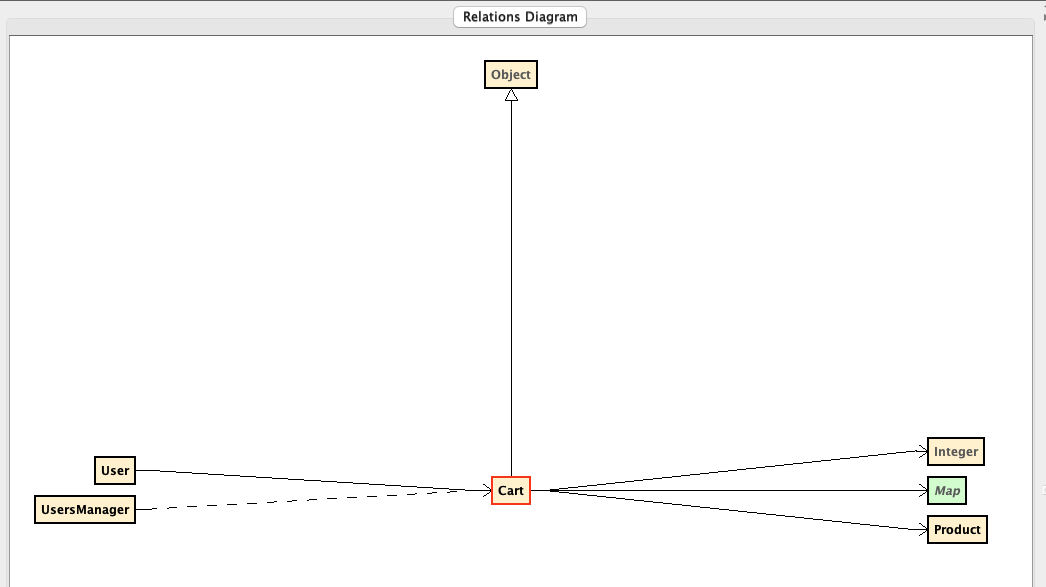
\includegraphics[width=0.5\textwidth]{img/cartDiagram.png}
\end{figure}
\begin{figure}[H]
    \centering
    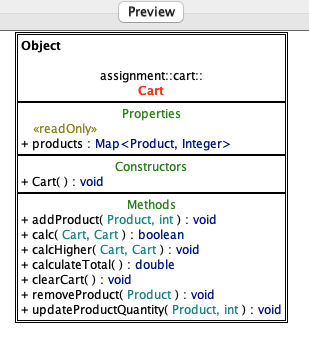
\includegraphics[width=0.5\textwidth]{img/cartPreview.png}
\end{figure}
\subsection{Product.java}
Uses: 1, Used by: 1
\begin{figure}[H]
    \centering
    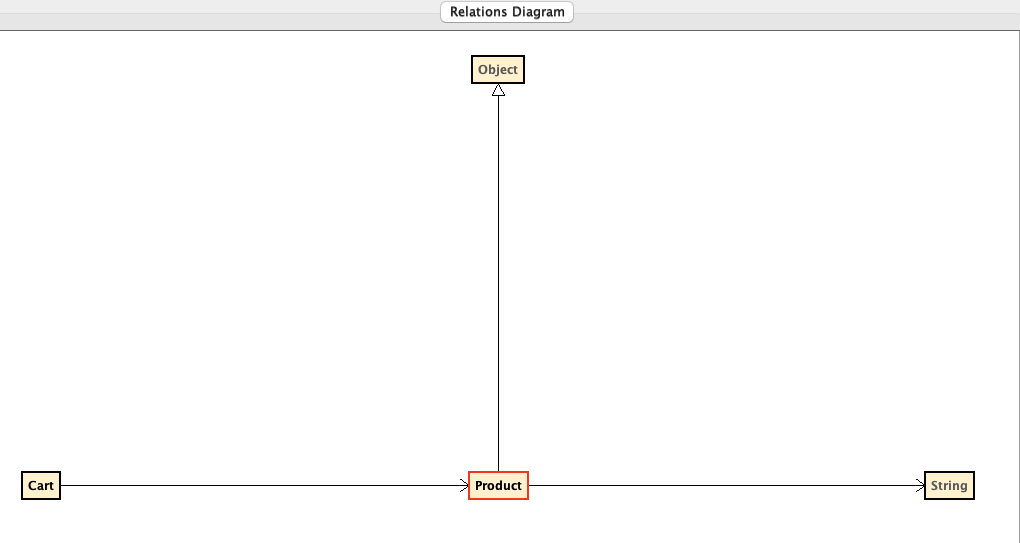
\includegraphics[width=0.5\textwidth]{img/productDiagram.png}
\end{figure}
\begin{figure}[H]
    \centering
    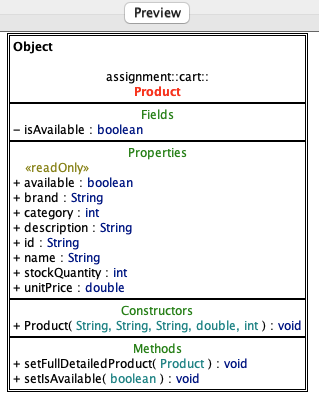
\includegraphics[width=0.5\textwidth]{img/productPreview.png}
\end{figure}
\subsection{User.java}
Uses: 4, Used by: 1
\begin{figure}[H]
    \centering
    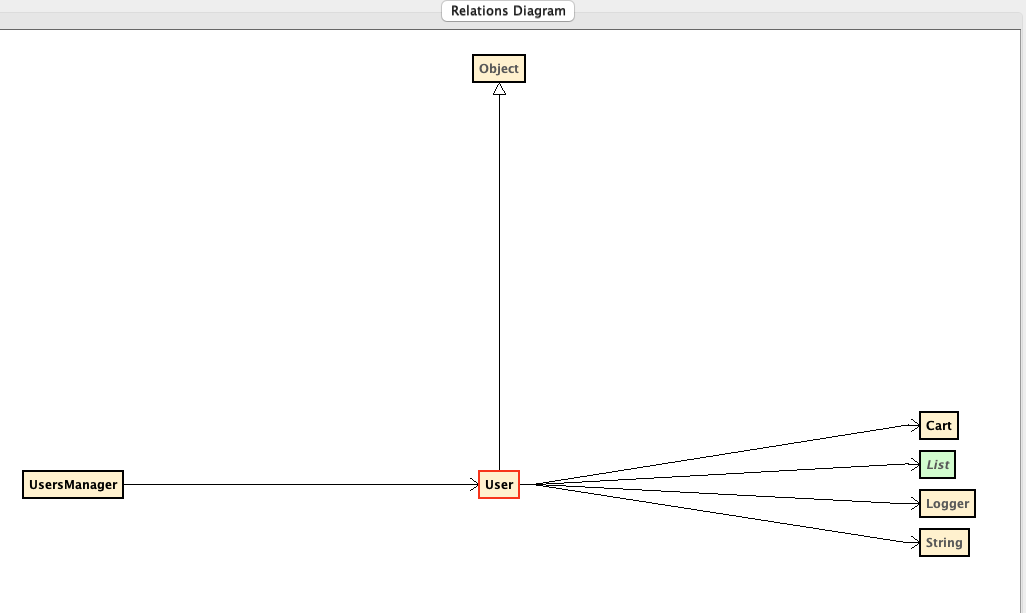
\includegraphics[width=0.5\textwidth]{img/userDiagram.png}
\end{figure}
\begin{figure}[H]
    \centering
    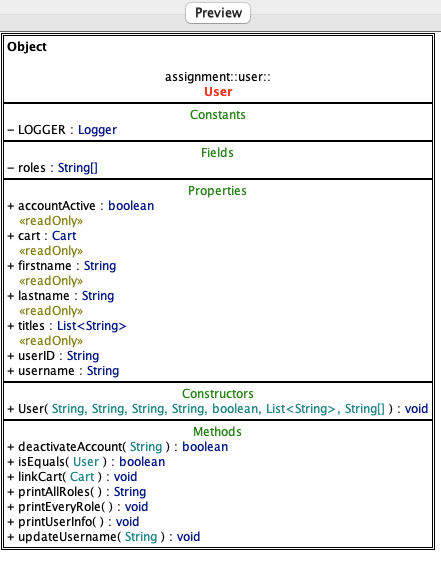
\includegraphics[width=0.5\textwidth]{img/userPreview.png}
\end{figure}
\subsection{UserManager.java}
Uses: 4, Used by: 0
\begin{figure}[H]
    \centering
    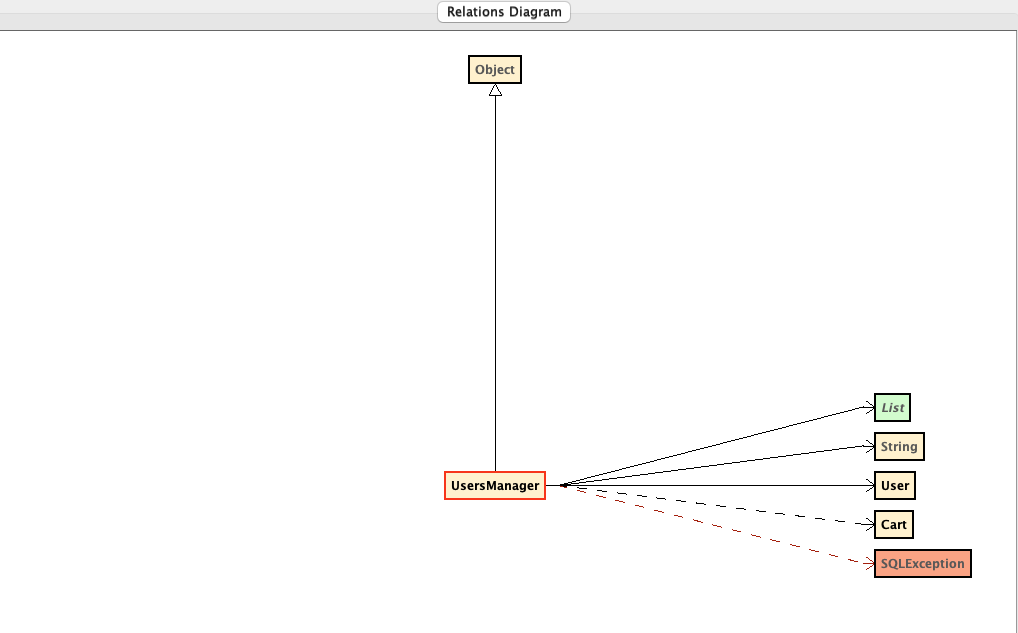
\includegraphics[width=0.5\textwidth]{img/userManagerDiagram.png}
\end{figure}
\begin{figure}[H]
    \centering
    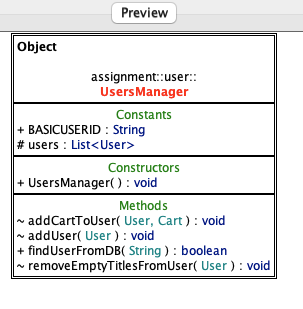
\includegraphics[width=0.5\textwidth]{img/userManagerPreview.png}
\end{figure}
\end{document}
